\documentclass[a4paper,12pt]{article}
\author{Firstname Lastname, Student number: 123456X}
\title{
CS-E5740 Complex Networks, \\
Answers to exercise set X
}
\pagestyle{empty}

% \usepackage{t1enc}
\usepackage{a4wide}
\usepackage{amsfonts}
\usepackage{verbatim}
\usepackage{amsmath}
\usepackage{amsfonts}
\usepackage{graphicx}
\usepackage[english]{babel}

\begin{document}
\vspace{8pt}

\maketitle

Compile with \verb!pdflatex ex_template.tex!

\section*{Problem 1}

\begin{itemize}
\item[a)] My answer to this question is...
\item[b)]
\end{itemize}





\clearpage

\section*{Problem 2}

\begin{itemize}

\item[a)] See Figure~\ref{fig:myfirstfig}.
\begin{figure}[h!]
\begin{center}
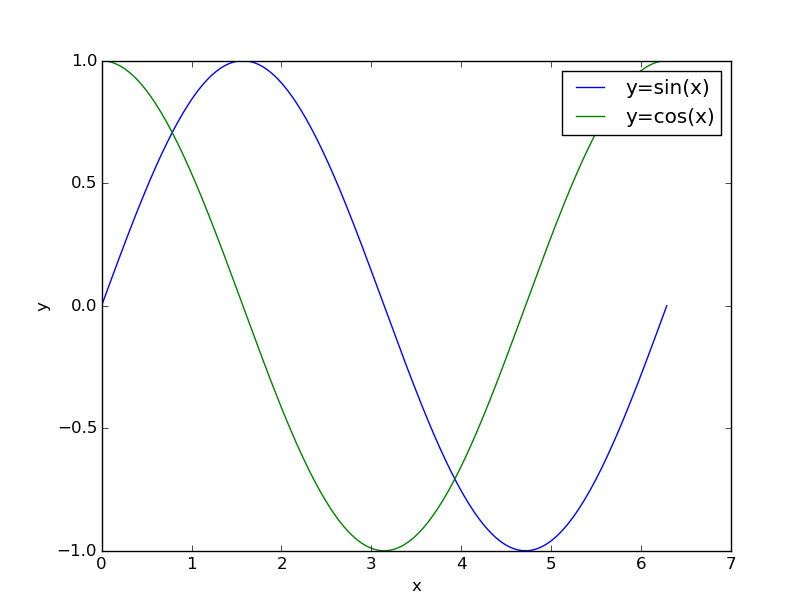
\includegraphics[width=0.5\textwidth]{example.png}
\caption{$\sin(x)$ and $\cos(x)$ are interesting functions.}
\label{fig:myfirstfig}
\end{center}
\end{figure}

\item[b)] ...

\end{itemize}

\clearpage


\end{document}
